\documentclass[10pt,a4paper]{article}
\usepackage[utf8]{inputenc}
\usepackage{amsmath}
\usepackage{amsfonts}
\usepackage{amssymb}
\usepackage{graphicx}
\usepackage{placeins}

\begin{document}
\section*{Piston Calculations}
\subsection*{Piston Ring Forces}
	\begin{figure}[h]
		\centering
		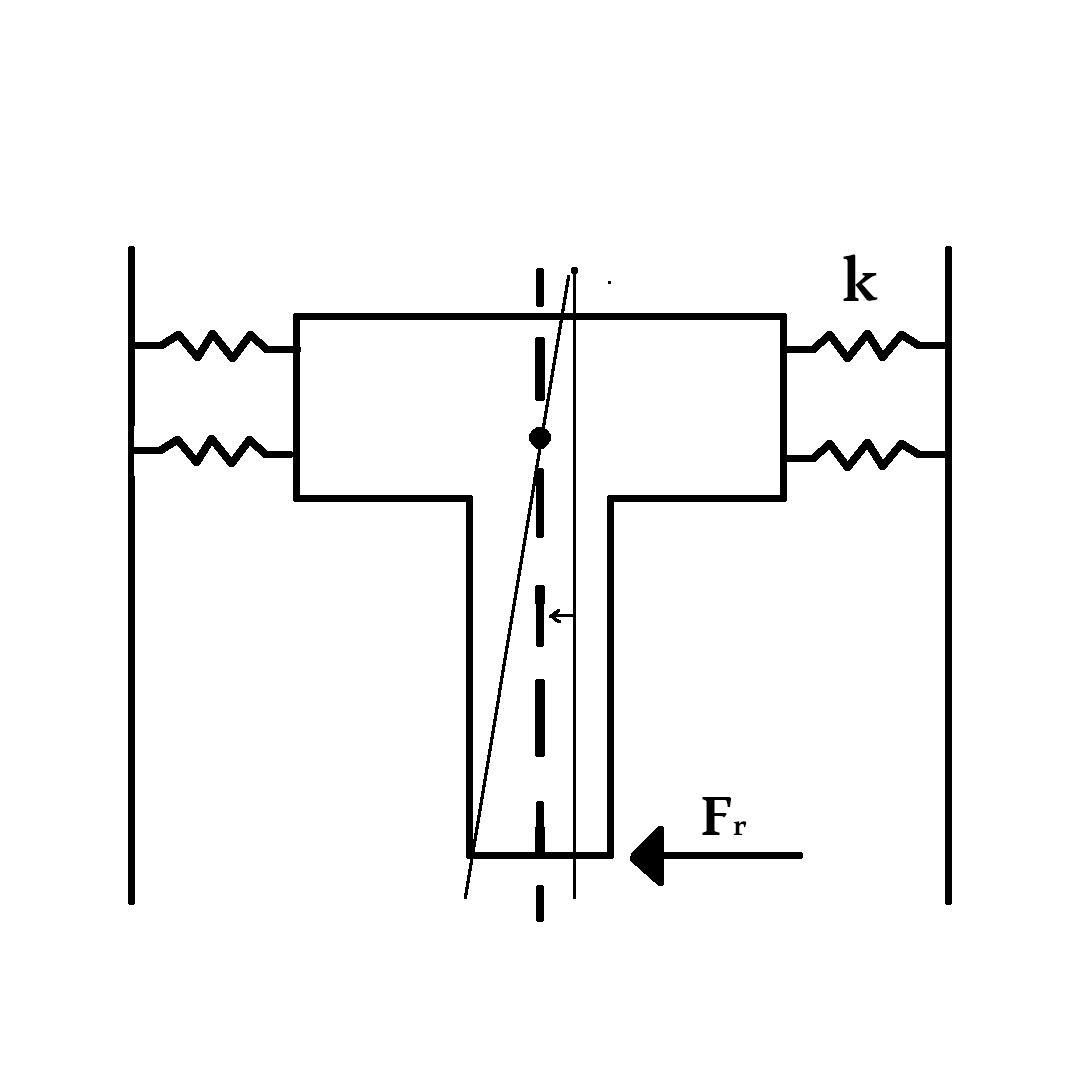
\includegraphics[width=.75\textwidth]{PistonDiagram.png}
		\caption{Ideal Gasket Forces}
		\label{fig:diagram1}
	\end{figure}
	The rings exhibit no vertical forces on the wall. Only the horizontal force from the connected rod is considered.
	The rings are simply modeled as springs connecting the piston to either side of the wall. Since the rings must maintain connection to the piston chamber wall, small deflections and angles are assumed. Thus small angle approximations are made.
	\begin{itemize}
	\item $\theta$ is the angle the piston is rotated with respect to the vertical.
	\item $x$ is the displacement of the piston.
	\item $z_{G_1}$ is the vertical distance from the top of the piston head to the center of the top ring.
	\item $z_{G_2}$ is the vertical distance from the top of the piston head to the center of the bottom ring.
	\item $z_{CG}$ is the vertical distance from the top of the piston head to the center of mass.
	\item $h_h$ is the height of the piston head.
	\item $d_h$ is the diameter of the piston head.
	\item $h_t$ is the height of the piston tail.
	\item $d_t$ is the diameter of the piston tail.
	\item $d_{go}$ and $d_{gi}$ is the inner and outer diameters of the rings.
	\item $h_g$ is the ring height.
	\item $\Delta t$ is the thickness of the rings, $\frac{d_{go}-d_{gi}}{2} $
	\end{itemize}
	First, the center of mass of the piston is calculated
	\begin{align}
		z_{CG} &= \frac{\frac{h_h}{2}d_h^2 h_h + (h_h+ \frac{h_t}{2}) d_t^2 h_t}{d_h^2 h_h + d_t^2 h_t }
	\end{align}
	
	The spring equation for the forces are written out.
	\begin{align}
		F_{G_{11}} &= k(x - (z_{CG}-z_{G_1}) \theta) \\
		F_{G_{12}} &= k(-x + (z_{CG}-z_{G_1}) \theta) \\
		F_{G_{21}} &= k(x - (z_{CG}-z_{G_2}) \theta) \\
		F_{G_{22}} &= k(-x + (z_{CG}-z_{G_2}) \theta) 
	\end{align}
	The moment and force equations are written out.
	\begin{align}
		F_R &= - F_{G_{11}} + F_{G_{12}} - F_{G_{21}} + F_{G_{22}}\\
		0 &= F_R (h_h + h_t - z_{CG}) + (F_{G_{12}} - F_{G_{11}})(z_{G_1} - z_{CG})+ (F_{G_{22}} - F_{G_{21}})(z_{G_2} - z_{CG})
	\end{align}
	Finally, x and theta are solved for.
	\begin{align}
	\alpha &= 2 h_{h} z_{CG} - h_{h} z_{G_1} - h_{h} z_{G_2} + 2 h_{t} z_{CG} - h_{t} z_{G_1} - h_{t} z_{G_2}\\
	\beta &= - 4 z_{CG}^{2} + 3 z_{CG} z_{G_1} + 3 z_{CG} z_{G_2} - z_{G_1}^{2} - z_{G_2}^{2}\\
		x &= \frac{F_{R} \left(\alpha +\beta\right)}{2 k \left(z_{G_1}^{2} - 2 z_{G_1} z_{G_2} + z_{G_2}^{2}\right)}\\
		\theta &= \frac{F_{R} \left(2 h_{h} + 2 h_{t} - 4 z_{CG} + z_{G_1} + z_{G_2}\right)}{2 k \left(z_{G_1}^{2} - 2 z_{G_1} z_{G_2} + z_{G_2}^{2}\right)}
	\end{align}
	The spring constant of the rings is derived in terms of material and geometric properties. To simplify calculation, the ring will be treated as a flat area cross section.
	\begin{align}
		\epsilon &= \frac{\sigma}{E}\\
		\Delta t &= t \epsilon = \frac{Pt}{A_C E} \\
		A_C &= d_{go} h_g \\
		k &= \frac{P}{\Delta t} = \frac{d_{go} h_g E}{\Delta t}
	\end{align}
	\subsection*{Ring Stresses and Pressures}
	The average pressure difference from the reaction forces is given below:
	\begin{align}
	 \Delta p_{G_X \text{avg}} &= \frac{F_{G_X}}{d_go h_g}
	\end{align}
	The minimum pressure which the rings must be fitted to is determined by the maximum pressure of the air $p_{AM}$ and the minimum change on pressure from the piston forces.
	\begin{align}
	p_{\text{fit}} &\geq p_{AM} - \frac{\text{min} \{ F_{G_X}, 0 \}}{d_{go} h_g}\\
	p_{\text{fit}} &= \frac{\Delta}{\frac{D_{hi}}{E_h} \Big( \frac{D_{ho}^2+D_{hi}^2}{D_{ho}^2-D_{hi}^2} + \nu_h \big) +\frac{D_{so}}{E_h} \Big( \frac{D_{so}^2+D_{si}^2}{D_{so}^2-D_{si}^2} + \nu_s \big) }
	\end{align}
	The radial ring stress is simply the pressure on the ring. Since the ring is thin walled, a constant radial stress is assumed.
	Since the rings are supported by the piston head, the tangential stress is derived using a thick walled pressure vessel equation, with a solid pressure vessel. Since the inner radius is 0, the resulting stresses are identical.
	\begin{align}
		\sigma_{gr} &= -p\\
		\sigma_{gt} &= -p
	\end{align}
	The pressures also attempts to push out the ring. The push out stress is derived below. The shear force is given pressure acting on the area of the ring directly exposed to the chamber.
	\begin{align}
	 V &= \frac{\pi}{4}(d_{go}^2-d_{h}^2) p\\
	 \tau_{\text{max}} &= \frac{3V}{2A} \\
	 \tau_{gp} &= \frac{3V}{2 h_g \pi \frac{d_h}{2} } = \frac{3 \pi (d_{go}^2-d_{h}^2) p}{4 h_g \pi d_h} 
	\end{align}
	Finally, friction creates a shear force on the ring. Since the ring reactions are equal and opposite, $p_{\text{avg}} = p_{\text{fit}}$.
	\begin{align}
		V &=  \mu p_{\text{avg}} A_o \\
		\tau_{\text{max}} &= \frac{3V}{2A_h} \\
		\tau_{f} &= \frac{3 \mu p_{\text{fit}} d_{go}^2}{d_h^2} 
	\end{align}
	The minimum and maximum of each ring stress is tabulated. Since the rings are fitted to compression, 
	\begin{align}
		\sigma_{gr\ \text{min}} &= \sigma_{gt\ \text{min}} = p_{\text{fit}} + \frac{\text{min} \{ F_{G_X}, 0 \}}{d_{go} h_g}\\
		\sigma_{gr\ \text{max}} &= \sigma_{gt\ \text{max}} = p_{\text{fit}} + \frac{\text{max} \{ F_{G_X}\}}{d_{go} h_g}\\
		\tau_{g\ \text{max}} &= \frac{3 \pi (d_{go}^2-d_{h}^2) p_{AM}}{4 h_g \pi d_h} - \frac{3 \mu p_{\text{fit}} d_{go}^2}{d_h^2}\\
		\tau_{g\  \text{min}} &= -\frac{3 \mu p_{\text{fit}} d_{go}^2}{d_h^2}
	\end{align}
	\subsection*{Axial Piston Stress Calculations}
	The axial force on the head is determined by the pressure. The resultant stress from the from the pressure in the piston major diameter is given below.
	\begin{align}
		\sigma_{z\ \text{Head}} &= - p
	\end{align}
	In the ring channels, a greater compression stress results from the smaller diameter and push out forces on the ring. Stress concentration factors $K_1$ and $K_2$ are added due to the geometry.
	\begin{align}
		\sigma_{z\ \text{Pressure}} &= - K_1 p \frac{d_h^2}{d_{gi}^2} \\
		\sigma_{z\ \text{Push Out}} &= - K_2 p \frac{d_{go}^2 - d_h^2}{d_h^2 - d_{gi}^2}\\
		\sigma_{z\ \text{Channel}} &= - K_1 p \frac{d_h^2}{d_{gi}^2} - K_2 p \frac{d_{go}^2 - d_h^2}{d_h^2 - d_{gi}^2}
	\end{align}
	The tail of the piston also has a concentration factor due to the diameter change, represented by $K_3$. The tail also experiences a stress concentration at the joint, which has a hole of diameter $d_j$ and concentration factor $K_4$.
	\begin{align}
		\sigma_{z\ \text{Tail}} &= -K_3 p \frac{d_h^2}{d_t^2}\\
		\sigma_{z\ \text{Joint}} &= - K_4 p \frac{d_h^2}{d_j^2}
	\end{align}
	Finally, a push out shear is present due to the joint. An upper limit is given by distributing the shear force among the smallest cross section.
	\begin{align}
		V &= \frac{F_R}{2}\\
		\tau &\leq \frac{3 F_R}{4 A_c}
	\end{align}
	The vertical deflection is estimated using $\delta = L \frac{\sigma}{E}$.
	\begin{align}
		\delta_{\text{Head}} &= - \frac{l_h p}{E}\\ 
		\delta_{\text{Tail}} &= - \frac{l_t p \frac{d_h^2}{d_t^2}}{E}\\ 
		\delta_{\text{Total}} &=  \frac{l_h p -l_t p \frac{d_h^2}{d_t^2}}{E}
	\end{align}
	Other than a negligible tensile force on the intake stroke, the piston is in compression in its entire loading cycle. Fatigue will be thusly ignored.
\end{document}